When analysing the  ZX diagram for a long staggered quantum walk (i.e. with more than 5 steps)  a pattern starts to emerge, repeating itself as many times as  the number of steps in the quantum walk. It seems able to represent, or at least to approximate, both the increment and decrement layers of the evolution operator. 
Its  ZX representation is

\begin{align*}
    \tikzfig{sqw-pattern-standard}
\end{align*}
\captionof{figure}{The alternative evolution operator for 3 qubits.}


\noindent
where $\alpha_n = \pm \frac{\pi}{4}$ and $\beta_n = \frac{2\pi}{3} + m\pi$, with $m=0$ or $m=1$.

There is also a slight variation of this operator, where a CNOT gate between the first and last qubit appears right after the $\beta_1$ Z-spider.


\begin{align*}
    \tikzfig{sqw-pattern-variation}
\end{align*}
\captionof{figure}{The variant of the alternative evolution operator for 3 qubits.}


This diagram does not fully capture the staggered model we started with, but, once suitably enveloped, it captures the exact same tensor as the original circuit. The set of gates to be placed as an envelope, in the beginning and the end of the diagram, does not exhibit a specific structure, but for 4 rotations combined with a seemingly random arrangement of other phase-less gates.

This construction appeared when optimising the 3 qubit staggered quantum walk. However, it can be  generalised for an $n$ qubit implementation,
 yielding the following operator, in the form of a ZX-diagram:

\begin{align*}
    \tikzfig{sqw-pattern-generalization}
\end{align*}
\captionof{figure}{The generalization of the alternative evolution operator for $n$ qubits.}


This operator is defined by entangling the first and last qubits and placing them in superposition. This is achieved by the XCX-gate (which is a CNOT with a Hadamard on both sides of the control),  followed by a CNOT gate between the first and last qubits and a rotation over the X-axis on the first one. Then follows a ladder of XCX-gates starting with the first qubit and the $n-1^{th}$ qubits and descending all the way to the second one. This is  followed by a rotation over the Z-axis along with a X-axis rotation. Then a CNOT is applied to the first and last qubits, followed by a X-axis rotation and a XCX-gate over the first qubit and the $n-1^{th}$ one. Finally, there is a second Z-axis rotation followed by the same ladder of XCX-gates, now appearing between the first and the $n-2^{th}$ qubits and descending all the way to the second; and, finally, a last X-axis rotation.

The rationale behind this operator is easy to explain: it creates a uniform distribution over a certain number of states, applies a rotation that makes some states more likely than others and then spreads these probabilities over the remaining states using CNOT gates. This also explains why the pattern 
 only shows up in staggered quantum walks over a certain length. The classical evolution operator resorting to the increment and decrement layers, needs to be repeated a number of times to be able to spread the probability distributions over the whole state space. This is what this version  does on the first layer. Thus, it cannot approximate staggered quantum walks with a small number of steps  as well as it can for longer ones.


%\subsection{Advantages of this alternative operator}

In any case, this alternative implementation has a number of advantages. First and foremost it reduces the total amount of gates needed to represent the evolution of the quantum walk. With the number of qubits increasing so does the cost of the increment and decrement layers, as a $n$ qubit staggered quantum walk needs to implement MCX gates with $n-1$ controls. Then, such MCX gates need to  be expanded into their basic gates representation \cite{gate-decomp}. The alternative operator uses gates controlled by at most 1 qubit. Moreover, to go from an $n$-qubit to an $n+1$ qubit quantum walk, all that needs to be done is to add two more XCX-gates, one to each ladder of XCX-gates. Such is not the case of the  evolution operator based on increment and decrement layers. 

In general, this makes the alternative operator much more efficient with respect to the total number of gates used, leading to lower depth  and, therefore, potentially less error-prone circuits.

As mentioned above, just by itself this operator is able of approximating the evolution of a staggered quantum walk. Although the approximation is not perfect it can yield results which are  quite similar to the ones obtained with the original implementation of the staggered model, as shown in the graph below.

\begin{align*}
    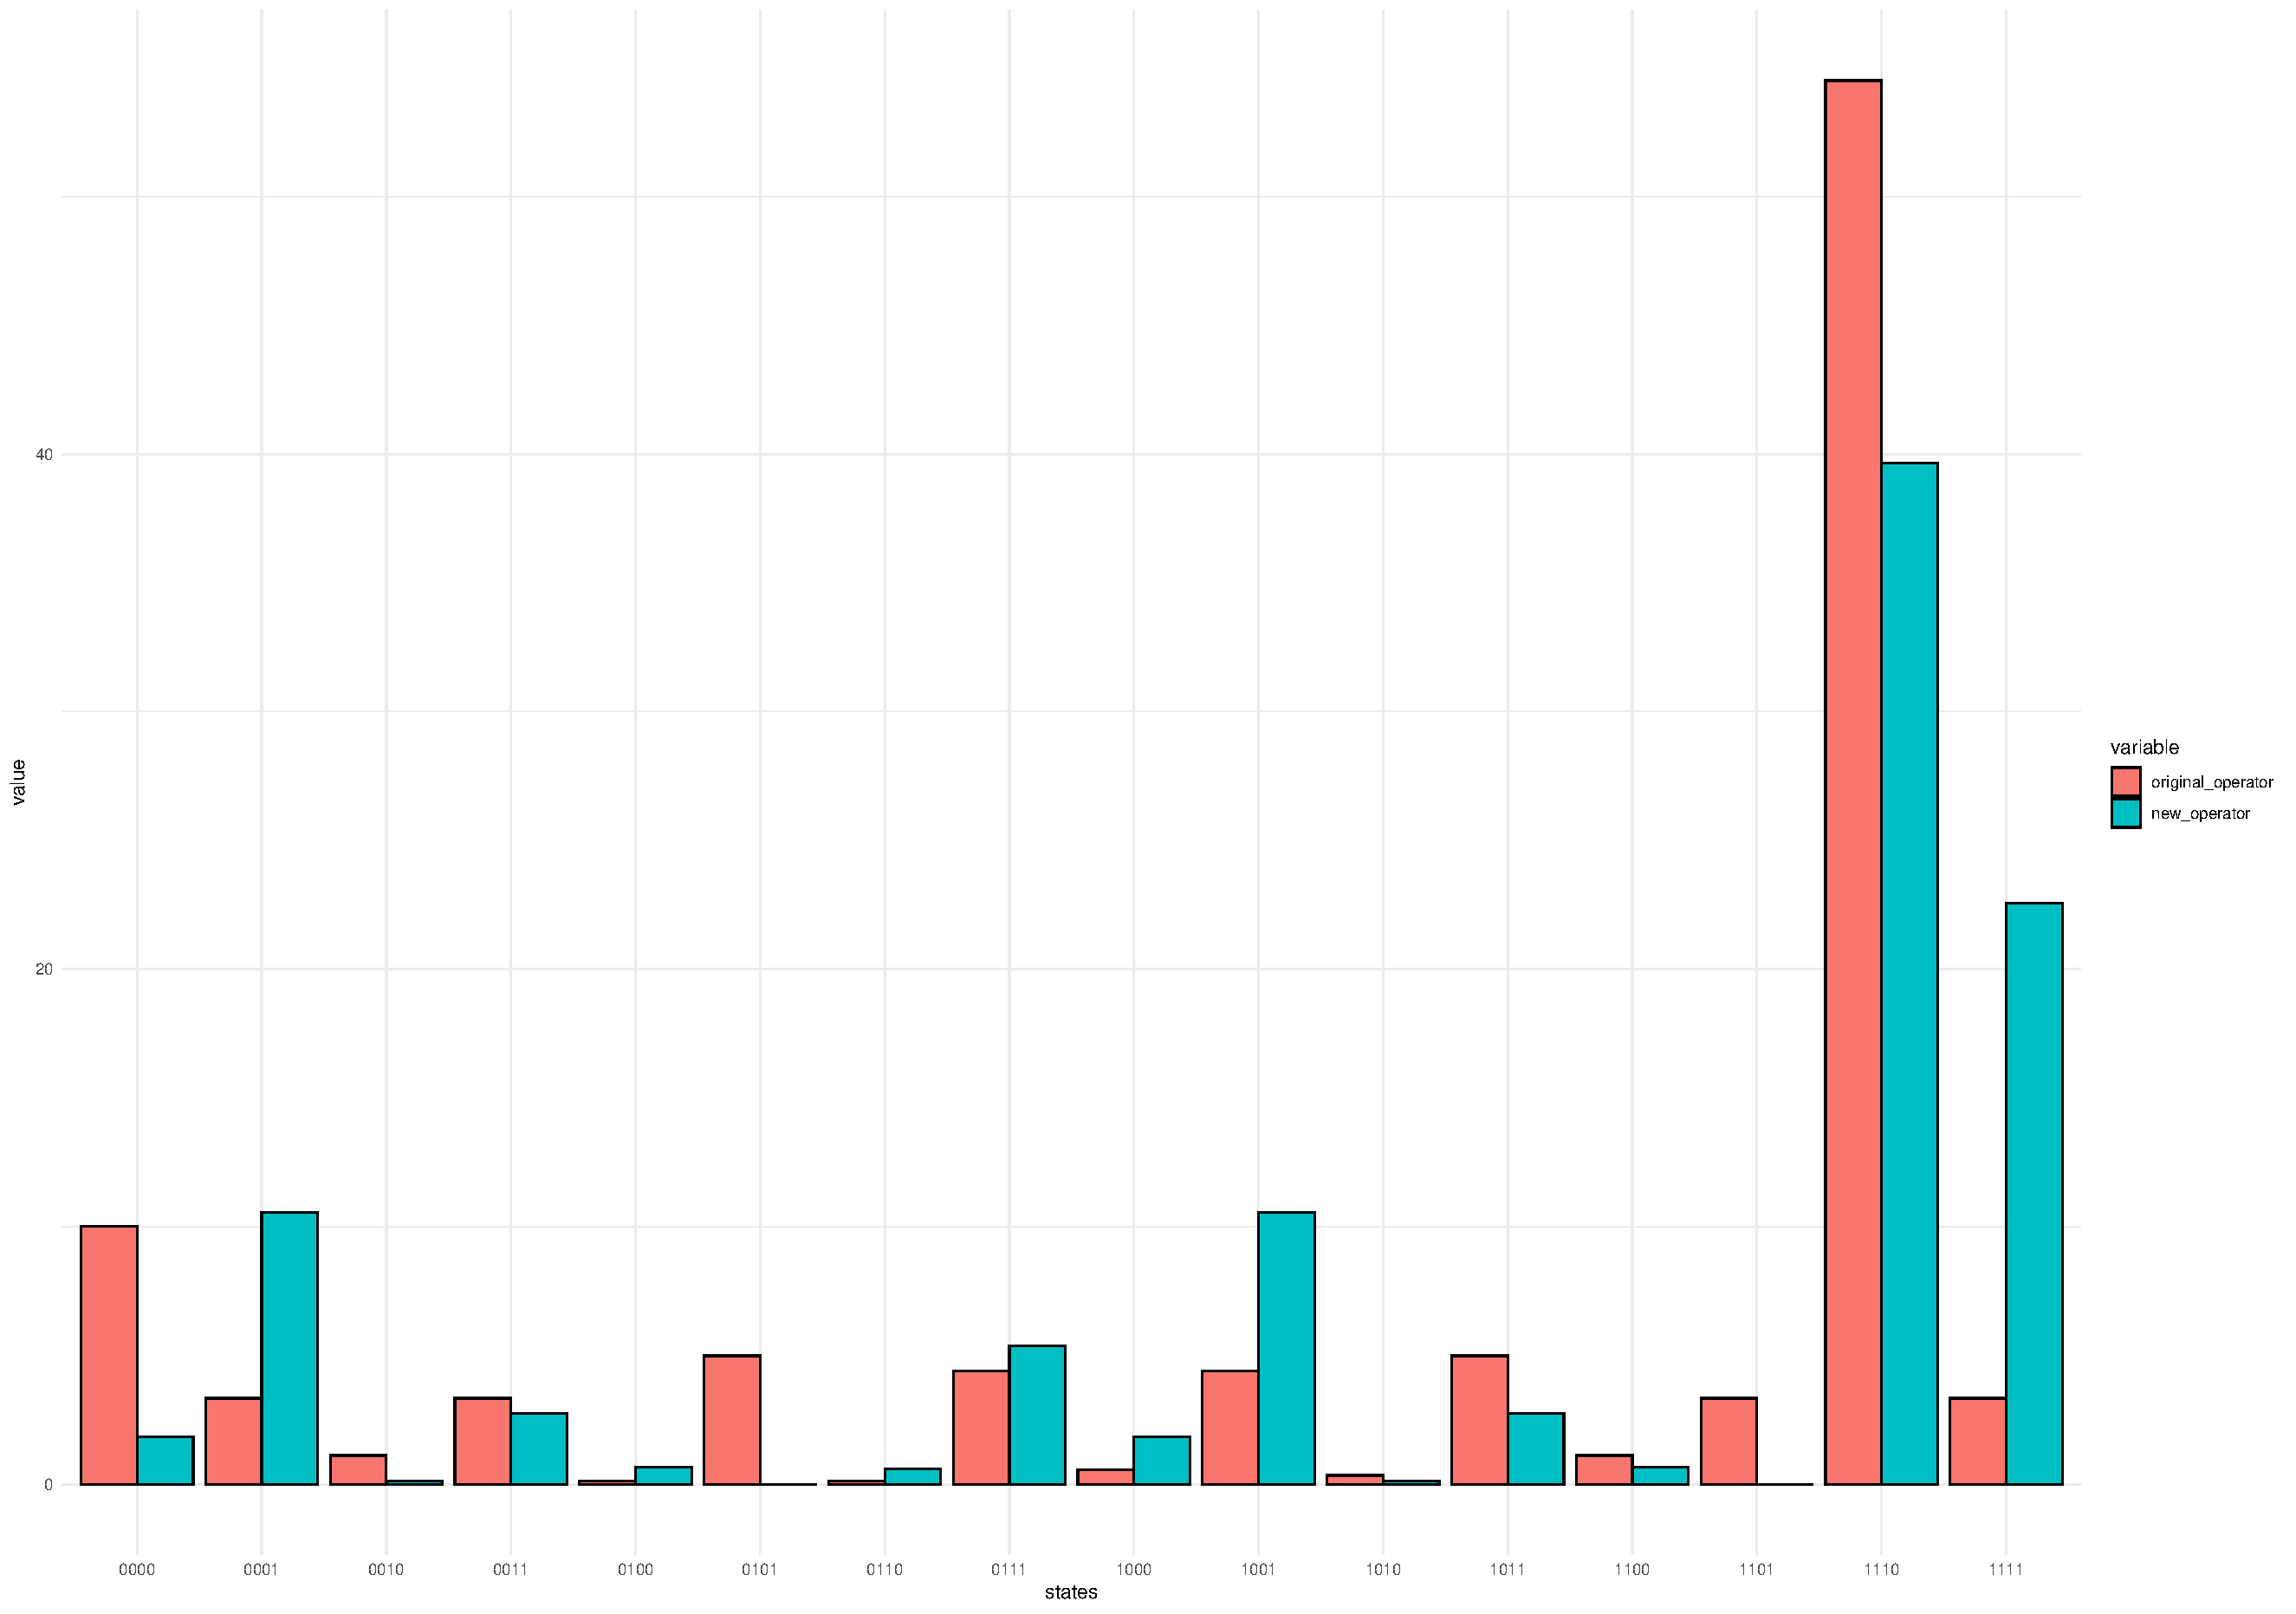
\includegraphics[width=0.7\linewidth]{figures/new_4step.pdf}
\end{align*}
\captionof{figure}{A comparison of the probabilities over the state space between the original evolution operator (red) and the alternative operator (blue) over 4 steps.}


One particular advantage of this alternative evolution operator is that it can work quite well on a quantum processor with  limited connectivity. This is due to the fact that all the qubits used in the staggered quantum walk only need to be strongly connected to  the first qubit, thus minimising possible errors occurring from having to operate on two qubits with poor connectivity.

However, a number of challenges remain, requiring further investigation. These concern the most suitable choice of parameters for $\alpha_n$ and $\beta_n$, as well as whether and how they depend on the number of qubits used in a particular staggered walk. Actually, when optimising the 4 qubit implementation of this circuit the resulting parameters did not seem to follow any regular pattern. 


%\subsection{Disadvantages of this alternative operator}

%Although this operator presents itself with a plethora of advantages it also presents a lot of challenges when it comes to actually using it. This is due mostly to the lack of reason as to which values should the $\alpha_n$ and $\beta_n$ parameters be. Or even, if these parameters should change with the change of how many qubits are used in the Staggered Quantum Walk. When optimizing the 3 qubit implementation of the SQW the resulting parameters did not seem to follow any reasonable pattern. 
%
%There doesn't seem to be a way to determine which values these parameters should take to approximate a given SQW.
%
%Also, there doesn't seem to be a guarantee as to if the next step of the SQW will be able to be approximated with the already established parameters, this can lead to sub-par approximations of the Staggered Quantum Walk.
%










